% PIR integrationstest

Der er fortaget en integrationstest imellem pir sensoren og pir API'en for at sikre at disse to interagerer korrekt sammen. Pir sensorens output er sat til P1(1) på PSoC'en, hvorefter der er brugt samme testprogram som i modultesten af pir API. Resultatet ses på figur \ref{lab:test_maaling1} og det kan nu konkluderes at pir sensor og pir API fungerer korrekt sammen, da ISR routinen går ind og aktiverer testpinen der måles på.

\begin{figure}[H]
\centering
{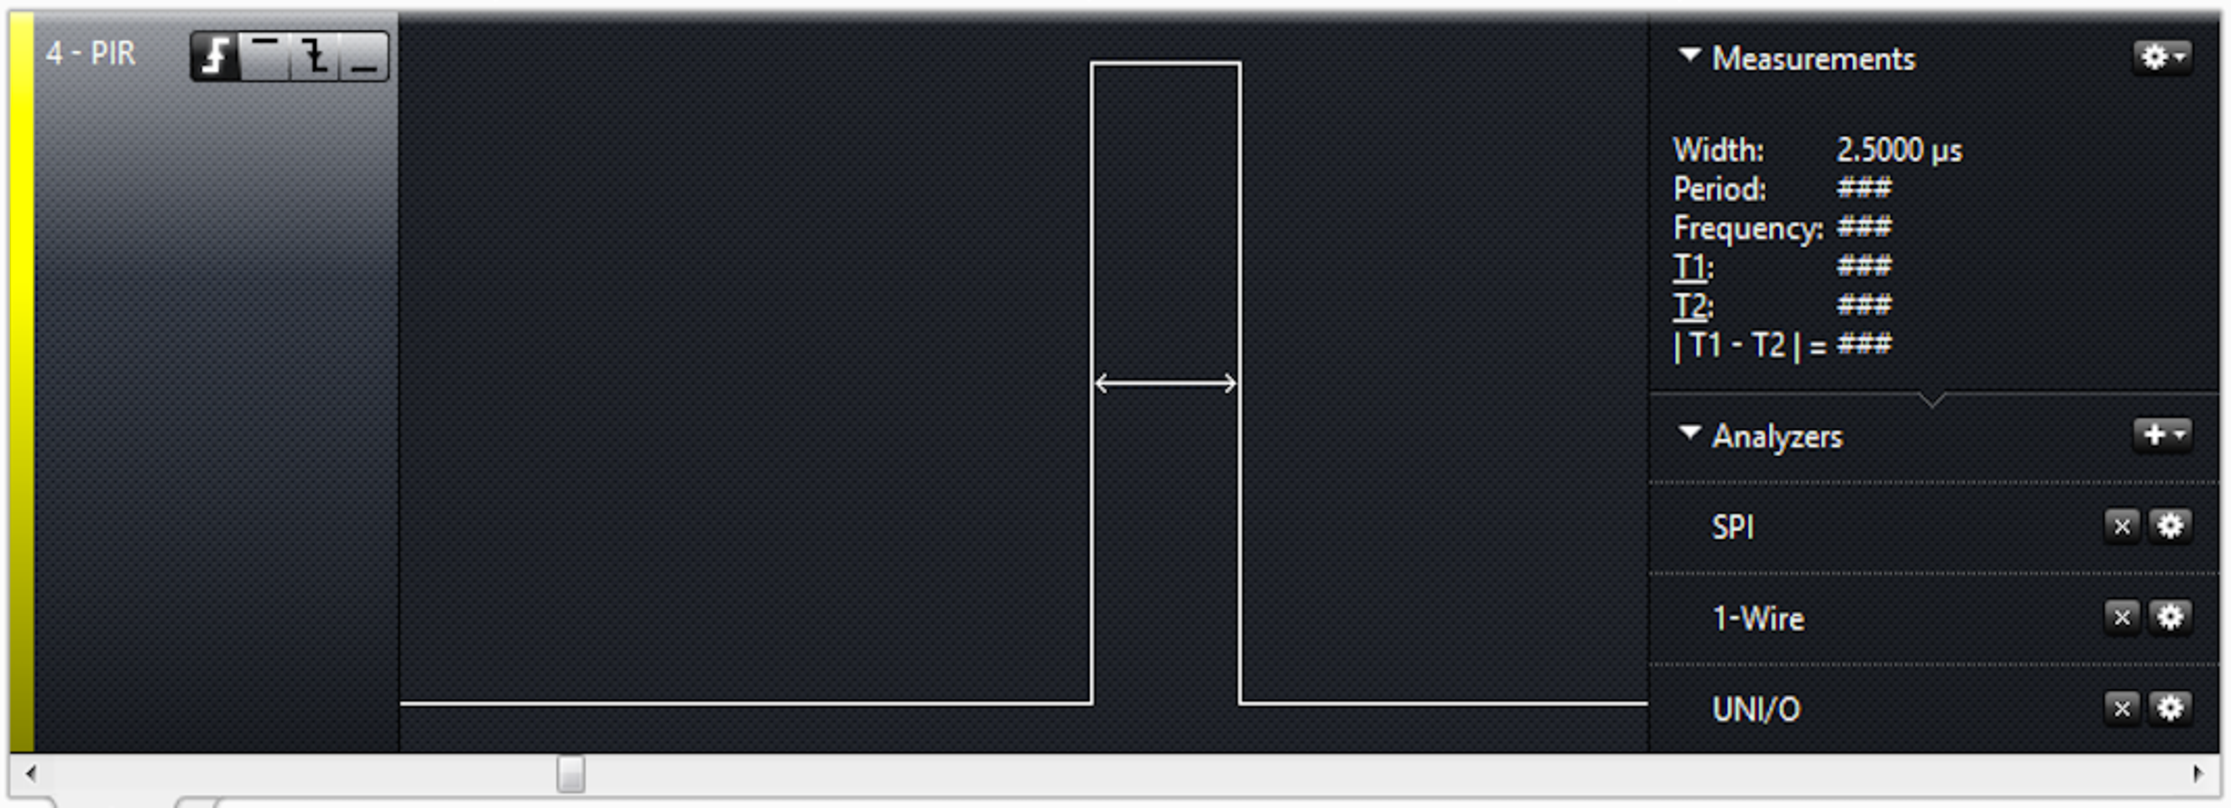
\includegraphics[width=0.60\textwidth]{filer/modultest/billeder/pir_testmaaling}}
\caption{Analyse billedet for pir aktivering}
\label{lab:test_maaling1}
\end{figure}  